\documentclass[oneside,a4paper,13pt]{book}

\usepackage[a4paper,inner = 1.7cm, outer = 2.7cm, top = 2cm, bottom = 2cm, bindingoffset = 1.2cm]{geometry}
\usepackage[french]{babel}
\usepackage{blindtext}
\usepackage[utf8]{inputenc} 
\usepackage[T1]{fontenc}
\usepackage{graphicx}
\usepackage{float}
\usepackage{geometry}
\geometry{hmargin=2.5cm,vmargin=1cm}
\usepackage{subfig}
\usepackage{lastpage}
\usepackage{fancyhdr}
\usepackage{blindtext}
\pagestyle{fancy}
\fancyhf{}
\cfoot{\thepage}

\usepackage{microtype}
\usepackage{amsmath}
\usepackage{amssymb}
\usepackage{index}
\usepackage{titlesec}
\usepackage{siunitx}


\lhead{BE de statistique}
\sisetup{detect-all = true}

\titleformat{\chapter}[display]
  {\Huge\bfseries}
  {}
  {0pt}
  {\thechapter.\ }
  
 \titleformat{name=\chapter,numberless}[display]
  {\Huge\bfseries}
  {}
  {0pt}
  {}



\begin{document}

\title{%
	BE Statistique \\ 
	\large FISE 1A}
\author{Nicolas Servot \\ Mathieu Pierronne}
\date{Juin 2020}

\maketitle



\chapter*{Exercice 1 : Nuisances sonores près d'un aéroport}

\paragraph{Question 1}

Le risque de la première hypothèse est que les habitants soient dédommagés injustement. \\
Le risque de la deuxième hypothèse est que les habitants soient dédommagés sans raison.

\paragraph{Question 2}

L'exercice consiste en l'étude d'un échantillon de taille 20 prélevé dans une population normale X d'écart-type $\sigma$ connu, mais de moyenne $\mu$ inconnue. Un test unilatéral sur la moyenne permet de tester les deux hypothèses $\mathcal{H}_{0}$ et $\mathcal{H}_{1}$. \\ 

 Sous l'hypothèse $\mathcal{H}_{0}$, supposant l'indépendance des variables $(X_{1},X_{2},...,X_{20})$ suivant la loi $\mathcal{N}(\mu_{0},\sigma^2)$, la densité de probabilité de $X := \sum_{i=1}^{20} X_{i}$ s'écrit : $\prod_{i=1}^{20} f_{0}(x_{i})$ \\

En appliquant le premier critère de Neyman et Pearson : $f_{1}(x)<\lambda f_{0}(x)$ on a:



\begin{align*}
    \frac{1}{(2\pi)^{10} \sigma^{20}} \exp(-\frac{1}{2}\sum_{k=1}^{20} \frac{(x_{k}-\mu_{1})^2}{\sigma^2}) &< \frac{\lambda}{(2\pi)^{10} \sigma^{20}} \exp(-\frac{1}{2}\sum_{k=1}^{20} \frac{(x_{k}-\mu_{0})^2}{\sigma^2}) \\
\intertext{En passant au logarithme naturel, et en posant $\overline{x}$ la moyenne empirique, il vient}
    \Leftrightarrow \;\;\; 2\overline{x}(\mu_{1}-\mu_{0}) - (\mu_{1}-\mu_{0})(\mu_{1}+\mu_{0}) &< \frac{2\sigma^2 ln(\lambda)}{20} \\ 
\intertext{On note $\overline{x_{c}}$ la limite a gauche de la region d'acceptation $w$,}
    \Leftrightarrow \;\;\; \overline{x_{c}} = \frac{\sigma^2 ln(\lambda)}{20(\mu_{1}-\mu_{0})} + \frac{(\mu_{1}+\mu_{0})}{2} &< \overline{x} \\ 
\intertext{La deuxième contrainte du test nous donne}
    P(\overline{X}<\overline{x_{c}}) &= \alpha = 0.05 \\
\intertext{où $\overline{X}$ est une variable aléatoire désignant la moyenne empirique de notre échantillon, tel que $\overline{X} \sim \mathcal{N}(\mu_{0}, \frac{\sigma}{\sqrt{20}})$.\newline
Afin de déterminer $\overline{x_{c}}$, on se ramène à une loi normale centrée réduite afin d'utiliser les tables de fonction de répartition. On a par les tables }\\
    P(\overline{X}<\overline{x_{c}}) &= \Phi \left( \frac{\overline{x_{c}} - \mu_{0}}{\sigma}\sqrt{20} \right)  \\
    \Rightarrow \;\;\; \overline{x_{c}} &\approx 78.85 \\
\end{align*} \\

\paragraph{Question 3} 

Afin d'exploiter et de calculer la moyenne empirique en dB de cet échantillon, on utilise la bibliothèque "csv" de python, qui nous permet de lire et manipuler de tels fichiers. \\

\begin{figure}[H]
\centering
  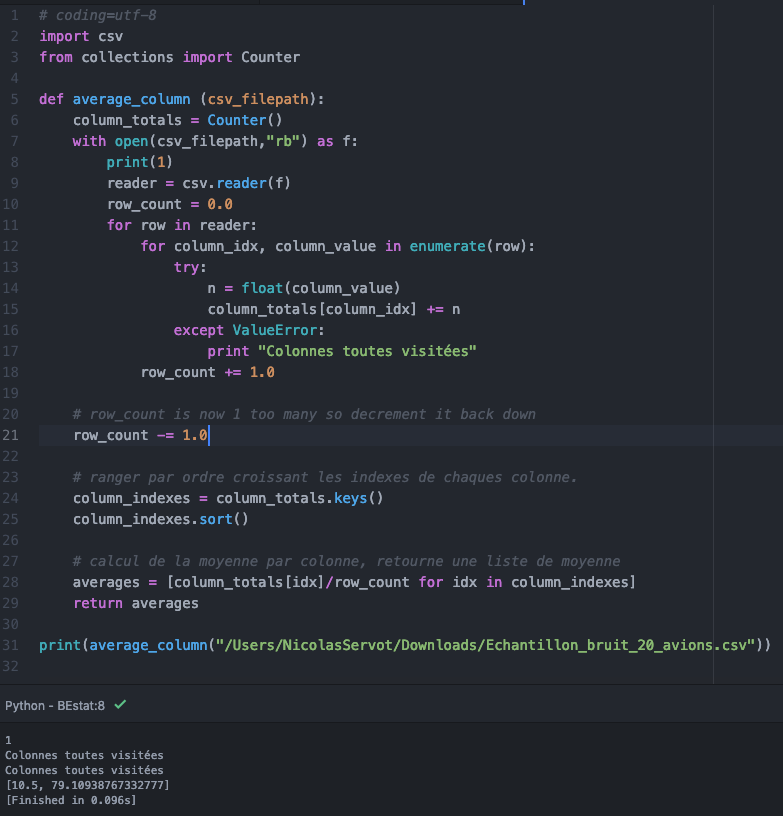
\includegraphics[width=0.8\linewidth]{src/q3.png}
  \caption{Script python calculant la moyenne demandée}
  \label{fig:q3}
\end{figure}

Le bruit moyen émis par ces 20 avions est de $\overline{M} = 79.1 dB$. Comme $M>\overline{x_{c}}$, l'hypothèse $\mathcal{H}_{0}$ n'est pas rejetée, les riverains sont donc dédommagés.

\paragraph{Question 4}

En reprenant le raisonnement inverse de la question 2, on cherche $\beta$ tel que

\begin{align*}
    \Phi \left( -\frac{\overline{x_{c}} - \mu_{1}}{\sigma}\sqrt{20} \right) &= \beta \\
\intertext{Par calcul, on a} 
    \frac{\overline{x_{c}} - \mu_{1}}{\sigma}\sqrt{20} &= 1.20 \\
\intertext{En repportant dans la table de $\mathcal{N}(0,1)$, il vient} 
    \beta &= 0.1151
\intertext{Finalement, la puissance du test $(1-\beta)$ est}
    1-\beta &= 0.8849
\end{align*}

\paragraph{Question 5}

Les 2 questions précédentes montrent que le risque de dédommager les habitants sans raison $\beta$ est 2 fois plus élevé que le risque de ne pas les dédommager à tord. Le test est donc biaisé et favorise les résidants.

\paragraph{Question 6}

En échangeant les deux hypothèses, la première condition de Neyman et Pearson devient

\begin{align*}
    \overline{x_{c}} = \frac{\sigma^2 ln(\lambda)}{20(\mu_{0}-\mu_{1})} + \frac{(\mu_{1}+\mu_{0})}{2} &> \overline{x} \\ 
\intertext{La deuxième contrainte du test nous donne}
    P(\overline{X}<\overline{x_{c}}) &= 1-\alpha = 0.95 \\
\intertext{où $\overline{X}$ est une variable aléatoire désignant la moyenne empirique de notre échantillon, tel que $\overline{X} \sim \mathcal{N}(\mu_{0}, \frac{\sigma}{\sqrt{20}})$.\newline
Afin de déterminer $\overline{x_{c}}$, on se ramène à une loi normale centrée réduite afin d'utiliser les tables de fonction de répartition. On a par les tables }\\
    P(\overline{X}<\overline{x_{c}}) &= \Phi \left( \frac{\overline{x_{c}} - \mu_{1}}{\sigma}\sqrt{20} \right) \\
    \Rightarrow \;\;\; \overline{x_{c}} &\approx 79.17 \\
\end{align*}

\begin{align*}
    \intertext{Le risque $\beta$ devient alors}
    \Phi \left( \frac{\overline{x_{c}} - \mu_{0}}{\sigma}\sqrt{20} \right) &= \beta \\
\intertext{Par calcul, on a} \\
    \frac{\overline{x_{c}} - \mu_{0}}{\sigma}\sqrt{20} &= -1.17 \\
\intertext{En repportant dans la table de $\mathcal{N}(0,1)$, il vient} 
    \beta &= 0.1210
\intertext{Finalement, la puissance du test $(1-\beta)$ est}
    1-\beta &= 0.8790
\end{align*}

Dans ce cas, $\overline{M} < \overline{X_{c}} = 79.17$, l'hypothèse $\mathcal{H}_{1}$ n'est pas rejetée, les habitants ne sont pas dédommagés.

\paragraph{Question 7}

L'ambiguité du test est exacerbée dans l'intervalle $I_{a}=[78.85,79.17]$. En effet, pour tout $\overline{m} \in I_{a}$, la décision d'indemnisation dépend de l'ordre des hypothèses $\mathcal{H}_{0}, \mathcal{H}_{1}$. \\ \\
Afin de résoudre ce problème, on pourrait fixer la limite $x_{c}$ telle que $x_{c}^{1} = x_{c}^{2}$. Une manière de s'y prendre est de poser $x_{c} = \frac{\mu_{0}+\mu_{1}}{2}$.

\paragraph{Question 8}

On a $\mathcal{P} \sim \text{Lognormal}(\lambda, \gamma^2)$. P admet un donc une densité de probabilité $p \longmapsto f(p,\lambda) = \frac{1}{p\gamma\sqrt{2\pi}}\exp\left(-\frac{(\ln{p}-\lambda)^2}{2\gamma^2}\right)$.\\ \\

La fonction de vraisemblance de lambda pour une telle loi est donc 

\begin{align*}
    \mathcal{L}(x,\lambda)  &= \prod_{i=1}^{n} f(p_{i},\lambda) \\
    \Leftrightarrow \;\;\; \mathcal{L}(x,\lambda)  &= \prod_{i=1}^{n} \frac{1}{p_{i}\gamma\sqrt{2\pi}}\exp\left(-\frac{(\ln{p_{i}}-\lambda)^2}{2\gamma^2}\right) \\
    \Leftrightarrow \;\;\; \mathcal{L}(x,\lambda)  &= \left(\frac{1}{\gamma\sqrt{2\pi}}\right)^n\prod_{i=1}^{n} \frac{1}{p_{i}}\exp\left(-\frac{(\ln{p_{i}}-\lambda)^2}{2\gamma^2}\right) \\
\intertext{En passant au log naturel}
    \Leftrightarrow \;\;\; \ln{\mathcal{L}(x,\lambda)}  &= -n\ln{\gamma\sqrt{2\pi}} -\sum_{i=1}^{n} \ln{p_{i}} -\frac{1}{2\gamma^2}\sum_{i=1}^{n} (\ln{p_{i}}-\lambda)^2 \\
\intertext{En dérivant par rapport à $\lambda$, il vient}
    \Leftrightarrow \;\;\; \frac{\partial\ln{\mathcal{L}(x,\lambda)}}{\partial\lambda}  &=\frac{1}{\gamma^2}\sum_{i=1}^{n}  \ln{p_{i}} - \lambda
\intertext{L'unique maximum est donc atteint pour $\widehat{\lambda} = \frac{1}{n}\sum_{i=1}^{n} \ln{p_{i}}$. $\widehat{\lambda}$ est l'estimateur du maximum de vraisemblance de $\lambda$.}
\end{align*}

\paragraph{Question 9}

\begin{align*}
\intertext{En remplaçant $\lambda$, par $\widehat{\lambda}$, on obtient l'estimateur des pertes moyennes $\mu_{p}$.}
    \mu_{p} &= \mathbb{E}(\mathcal{P}, \widehat{\lambda}) \\
    \Leftrightarrow \;\;\; \mu_{p} &= e^{\frac{\gamma^2}{2}}\left(\prod_{i=1}^{n} p_{i}\right)^\frac{1}{n}
\end{align*}


\paragraph{Question 10}
Sur le logiciel R, on réalise le code suivant : 

\begin{figure}[H]
\centering
  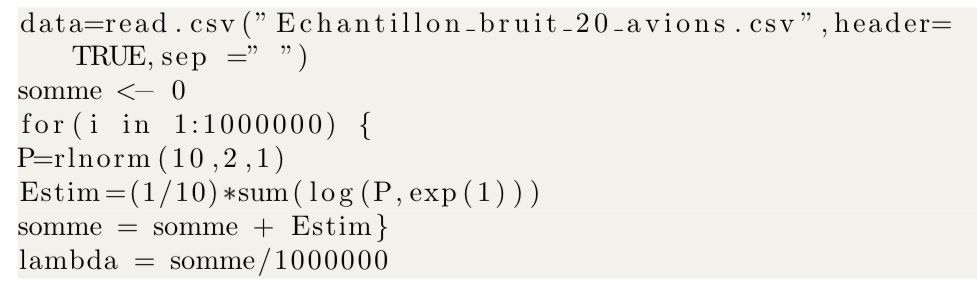
\includegraphics[width=0.8\linewidth]{src/q10-1.jpg}
  \caption{Script python calculant la moyenne demandée}
  \label{fig:q3}
\end{figure}

On obtient le résultat suivant : 
\begin{figure}[H]
\centering
  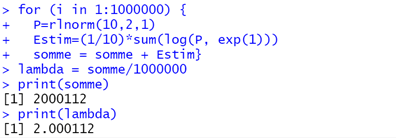
\includegraphics[width=0.8\linewidth]{src/q10-2.png}
  \caption{Script python calculant la moyenne demandée}
  \label{fig:q3}
\end{figure}
Sur 10 échantillons, l'écart entre la moyenne et l'estimateur est négligeable (il est de seulement 0,0000112). Expérimentalement, l'estimateur $\widehat{\lambda}$ n'est pas biaisé.

\paragraph{Question 11}

Afin de prendre en compte les fluctuations P, on peut étudier une nouvelle variable aléatoire $Y = X-P$.

\chapter*{Exercice 2 : Qualité de l’air}

\paragraph{Question 1}
Si la qualité de l'air semble être beaucoup plus variable dans les villes côtières, la valeur médiane y est plus faible. En effet, la médiane est de 85 pour les villes côtières contre 124 pour les villes non côtières. Malgré, le fort espacement des valeurs en villes côtières (l'écart type de la qualité de l'air est de 28 pour les villes côtières contre 10 pour les villes non côtières), je préférerais vivre dans les villes côtières car la valeur médiane de la qualité de l'air y est beaucoup plus faible qu'en zone non côtière. L'air y est donc plus pur. 

\begin{figure}[h]
  \centering
  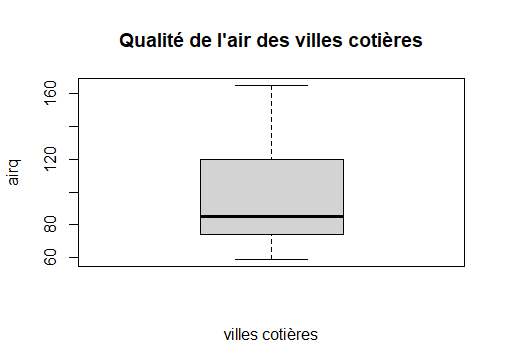
\includegraphics[width=0.4\textwidth]{Images/Qaircot.png}\label{fig:f1}
  \hfill
  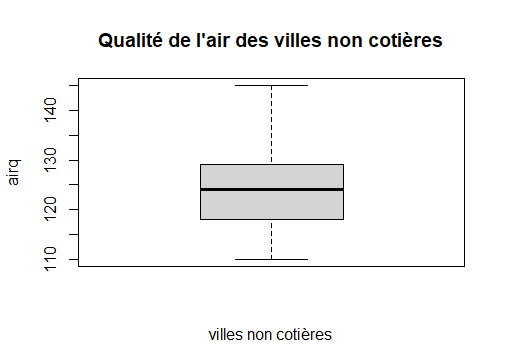
\includegraphics[width=0.4\textwidth]{Images/Qairnoncot.png}\label{fig:f2}
  \caption{Répartition de la qualité de l'air en villes côtières et non côtières}
\end{figure}

\paragraph{Question 2.a}
Nous souhaitons, dans cette question, utiliser un test de comparaison de populations normales pour valider ou non l’hypothèse selon laquelle le salaire moyen des habitants des métropoles côtières se distribue de façon équivalente à celui des villes plus éloignées des côtes. Nous alors essayer de déterminer si l'hypothèse d'égalités moyennes est vérifiée sur ces deux échantillons. 

\smallbreak
Pour cela, nous devons avant tout vérifier que l'hypothèse d'égalité des variances n'est pas rejetée. 
Nous devons alors comparer les variances en faisant l'hypothèse $\mathcal{H}_{0}$ : $\sigma_{a}$=$\sigma_{b}$ (avec a et b les deux échantillons étudiés) et l'hypothèse alternative $\mathcal{H}_{1}$ : $\sigma_{a}$\neq$\sigma_{b}$. Il s'agit donc d'un test bilatéral. On a : 

\begin{align*}
    F = \frac{n_{a}S_{a}^{2}/(n_{a}-1)}{n_{b}S_{b}^{2}/(n_{b}-1)}=\frac{21\times8S_{a}^{2}}{20\times9S_{b}^{2}}\sim \mathcal{F}(20,8)
\end{align*}

Nous pourrons ensuite faire l'hypothèse d'égalité des moyennes avec l'hypothèse $\mathcal{H}_{0}$ : $\mu_{a}$=$\mu_{b}$  et l'hypothèse alternative $\mathcal{H}_{1}$ : $\mu_{a}$\neq$\mu_{b}$. Sous $\mathcal{H}_{0}$, on a : 

\begin{align*}
    T = \frac{\overline{X_{a}}-\overline{X_{b}}}{S^{*}\sqrt{\frac{1}{n_{a}}+\frac{1}{n_{b}}}} 
    = \frac{\overline{X_{a}}-\overline{X_{b}}}{S^{*}\sqrt{\frac{1}{21}+\frac{1}{9}}} \sim \mathcal{T}(n_{a}+n_{b}-2=28)
\end{align*}

Si ces deux hypothèses sont validées, nous pourrons affirmer que le salaire moyen des habitants des métropoles côtières se distribue
de façon équivalente à celui des villes plus éloignées des côtes.

\paragraph{Question 2.b}
\textit{var.test} permet de comparer la variance de deux groupes d'échantillon ayant une distribution normale. Ici, la distribution des deux groupes est supposée normale. Par conséquent, la fonction \textit{var.test} peut être utilisée. 
\smallbreak
\textit{t.test} sert à comparer la moyenne de deux groupes. Elle peut être utilisée si les deux groupes sont échantillonnée à partir de distribution normale avec des variances égales. Nous verrons dans la question 2.c) que l'hypothèse d'égalité des variances ne peut être rejetée. Nous pouvons ainsi supposer les variances égales et utiliser la fonction \textit{t.test}.\\
Par conséquent, dans les conditions de l'énoncé, on peut utiliser ces deux fonctions R car les populations étudiées sont considérées comme normales et que l'hypothèse d'égalité des variances est validée. 

\paragraph{Question 2.c}
Tout d'abord, l'hypothèse d'égalité des variances nous donne : 
\begin{align*}
    F = \frac{21\times8S_{a}^{2}}{20\times9S_{b}^{2}}\sim \mathcal{F}(20,8)
\end{align*}

En utilisant les tables de Fisher-Snedecor, la région critique au risque de 5\% est définie par\\ f < 0,34 et f > 4. \\
De plus, d'après la question précédente, nous pouvons utiliser la fonction la fonction \textit{var.test} qui nous donne directement f = $\frac{s_{a}^{2}}{s_{b}^{2}}$ = 1,7715. 
f ne se trouve donc pas dans la région critique : on ne peut pas alors rejeter l'hypothèse d'égalité des variances. 

\smallbreak
On fait maintenant l'hypothèse d'égalité des moyennes, $\mathcal{H}_{0}$ : $\mu_{a}$=$\mu_{b}$. L'hypothèse alternative est $\mathcal{H}_{1}$ : $\mu_{a}$\neq$\mu_{b}$. Sous $\mathcal{H}_{0}$, on a : 

\begin{align*}
    T = \frac{\overline{X_{a}}-\overline{X_{b}}}{S^{*}\sqrt{\frac{1}{21}+\frac{1}{9}}} \sim \mathcal{T}(n_{a}+n_{b}-2=28)
\end{align*}

En utilisant les tables de Student, la région critique au risque de 5\% est définie par|t| > 2,048. \\
Or la fonction \textit{t.test} du logiciel R nous donne t = 1,0229. t étant inférieur à 2,048, il n'est pas dans la région critique. On ne peut donc pas rejeter l'hypothèse $\mathcal{H}_{0}$. On en conclue qu'il n'y a pas de différence significative entre les deux moyennes et que la distribution des salaires moyens dans les métropoles côtières est équivalente à la distribution des salaires dans les villes plus éloignées des cotes. 

\paragraph{Question 2.d}
Tous les résultats établis précédemment reposent sur une hypothèse initiale : la distribution des deux échantillons est normale. \\
Cependant, cette affirmation n'est pas forcement juste. Nous allons alors, à l'aide de la fonction \textit{qqnorm} sur R, comparer les quartiles des deux échantillons aux quartiles de la loi normale. On trace ces deux fonctions pour respectivement les villes côtières et non côtières. On obtient les deux graphes suivants : 

\begin{figure}[H]
  \centering
  \subfloat[Ville côtières]{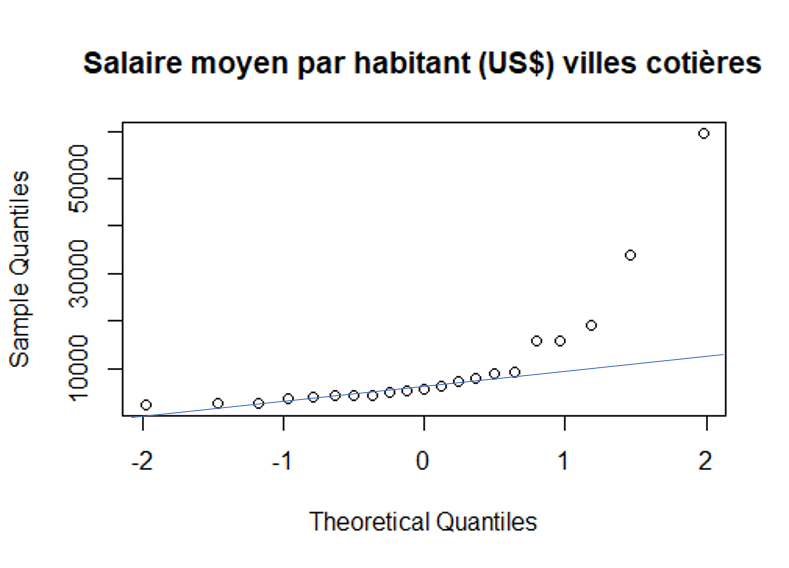
\includegraphics[width=0.4\textwidth]{Images/normaleCot2.png}\label{fig:f1}}
  \hfill
  \subfloat[Villes non côtières]{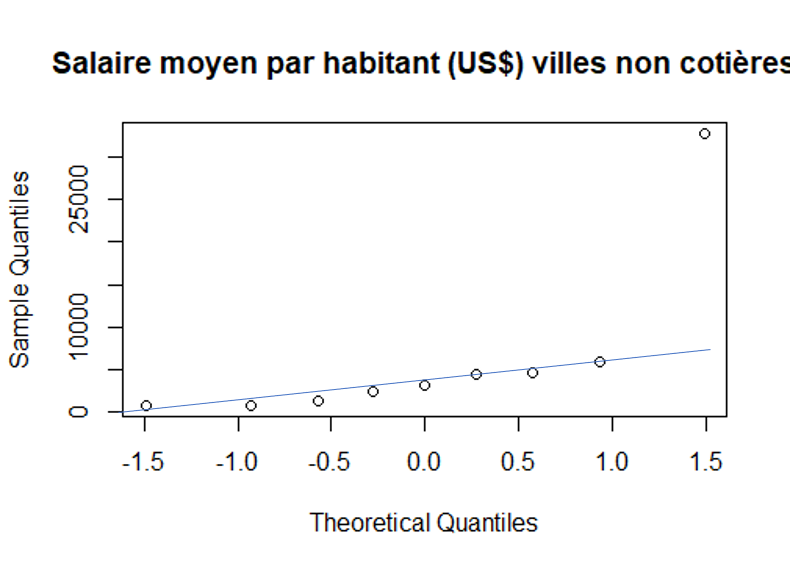
\includegraphics[width=0.4\textwidth]{Images/normalenonCot2.png}\label{fig:f2}}
  \caption{Lien entre les quartiles d'une loi normale et des quartiles des échantillons étudiés}
\end{figure}

Si on observe une relation affine entre les quartiles des salaires des habitants des villes non côtières et les quartiles de la loi normale, on ne retrouve pas cette dépendance linéaire pour les villes côtières. Par conséquent, si nous pouvons supposer que les salaires des habitants des villes non côtières suit une loi normale, cette hypothèse n'est pas juste pour les villes côtières. Les résultats établies dans les questions précédentes sont donc à prendre avec précaution. 

\paragraph{Question 3}
On trace à l'aide du logiciel R, les données de bonne santé des entreprises en fonction du salaire moyen des habitants. La bonne santé des entreprises est représenté par la valeur ajouté créée par l'entreprise en millier d'euros (vala). On obtient le graphe suivant avec en rouge les villes non côtières et bleu les villes côtières  :
 
\begin{figure}[H]
\centering
  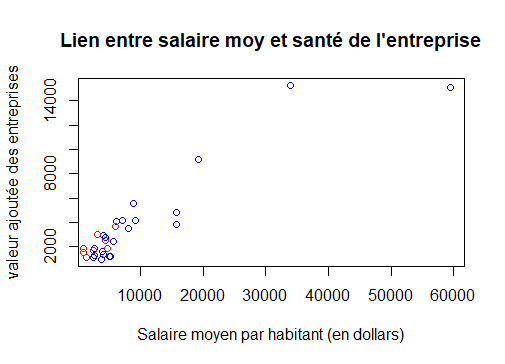
\includegraphics[width=0.8\linewidth]{Images/sante.png}
  \caption{Données de bonne santé des entreprises en fonction du salaire moyen des habitants}
  \label{fig:q3}
\end{figure}

Il existe donc une relation linéaire entre le salaire moyen des habitants et la valeur ajoutée des entreprises. En effet, on observe que plus le salaire moyen des habitants est élevé, plus les entreprises sont en bonnes santé et la valeur ajoutée des entreprises est élevée. 

\paragraph{Question 4}
Le graphe établie à la question 3 nous montre bien qu'il y a un lien de corrélation entre le salaire des habitants et la santé des entreprises d'une ville. Cependant, ce n'est pas parce qu'il y a un lien de corrélation entre ces deux éléments, qu'il y a un lien de causalité. \\
Par exemple, en France 57 \% des morts ont lieu à l’hôpital : la probabilité de mourir dans les établissements de santé est supérieure à celle de passer l’arme à gauche chez soi dans son lit. Pourtant l'hopital n'est pas un lieu plus dangereux que notre belle maison. Si la proportion de morts est plus élevée à l’hôpital, c’est parce qu’on s’y rend lorsqu’on est malade, et que c’est quand on est malade qu’on risque le plus de mourir. Il y a une différence entre corrélation et causalité. 
\smallbreak
Par conséquent, il n'y a pas forcément de causalité entre le salaires des habitants et la santé des entreprises d'une ville : augmenter les salaires des habitants n'aura forcément pour effet d’améliorer la santé des entreprises 

\end{document}
